\section{Experiments}\label{sec:experiments}

We now seek to empirically assess our proposed approach for active testing of LLMs (\Cref{sec:scaling_method}), as well as our proposed risk-error-estimation method (\Cref{sec:error_estimation_method}).
We provide implementation details in \Cref{sec:experiment_details} and code at \shorturl{github.com/gabrielleberrada/scaling-up-active-testing}.


\subsection{Setup}\label{sec:experimental_setup}

We use five text-classification datasets: Stanford Sentiment Treebank 2 (SST-2; \citealp{socher2013recursive}), Subjectivity (Subj; \citealp{pang2004sentimental}), Financial Phrase Bank (FPB; \citealp{malo2013good}), Hate Speech (HS; \citealp{degibert2018hate}) and Massive Multitask Language Understanding (MMLU; \citealp{hendrycks2021measuring}).
We mainly focus on the first four, which were previously used by \citet{kossen2024context}, then use MMLU to explore a problem that is more challenging for the models used in our experiments.

The models we use span three model families and have parameter counts ranging from 1 to 70 billion.
In our main experiments we use the 7B and 70B versions of Llama 2 \citep{touvron2023llama} along with Gemma3-4B \citep{kamath2025gemma}; in additional experiments we use Phi-2 \citep{javaheripi2023phi} and Gemma3-1B.
We use these models with either zero- or few-shot prompting, with both including appropriate task prompting such as ``Classify the sentiment of the following sentence as positive or negative''.
We denote our four Llama 2 model configurations as 7B-zero, 70B-zero, 7B-few and 70B-few, and our two Gemma 3 model configurations as Gemma3-4B-zero and Gemma3-4B-few.

\begin{figure*}[t]
    \begin{subfigure}[b]{\linewidth}
        \centering
        % trim={<left> <lower> <right> <upper>}
        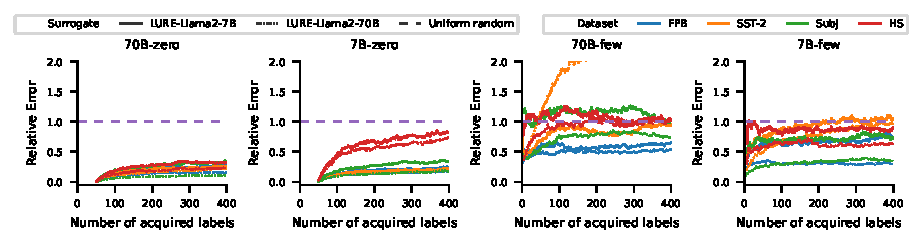
\includegraphics[width=\linewidth,trim={8pt 5pt 0 0}]{
            figures/pdf/70b_7b_zeroshot_fewshot_relative_error.pdf
        }
        \caption{Llama 2 target models and Llama 2 surrogate models}
         \label{fig:7b_70b_llama_unif_lure}
    \end{subfigure}
    \begin{subfigure}[b]{\linewidth}
        \centering
        % trim={<left> <lower> <right> <upper>}
        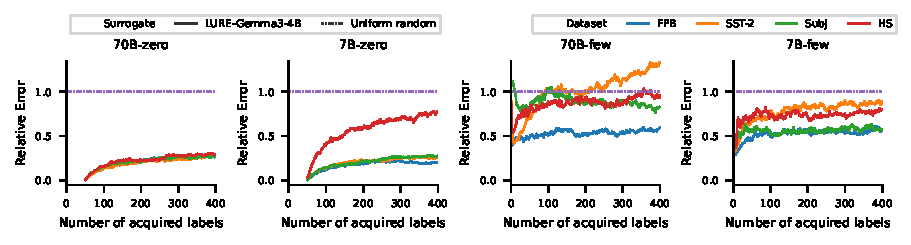
\includegraphics[width=\linewidth, trim={5pt 5pt 0 0}]{
            figures/pdf/relative_errors_gemma.pdf
        }
        \caption{Llama 2 target models and Gemma3-4B surrogate model}
        \label{fig:7b_70b_gemma_unif_lure}
    \end{subfigure}
    \caption{
        Cheap surrogate models support effective data acquisition for active testing.
        We compare uniform-random testing to active testing (LURE) across four datasets.
        To guide active data acquisition we use a surrogate model that we train using a single step of in-context learning and then keep fixed.
        This stripped-back surrogate-model training, along with the use of small surrogate models relative to the target models, allows us to drastically reduce the computational cost of active testing while achieving strong performance.
    }
    \label{fig:7b_70b_zeroshot_fewshot_unif_lure}
    \vspace{-8pt}
\end{figure*}


We compare active testing to uniform-random testing, a standard approach to model evaluation.
Acquisition methods from the active-learning literature \citep{settles2012active} are not tailored for risk estimation \citep{kossen2021active} and so would have limited utility as baseline methods here.

We use a logarithmic loss, as discussed in \Cref{sec:background,sec:scaling_method}. 
Like in past work \citep{kossen2021active,kossen2022active}, we measure the performance of a testing method using the median squared error of its risk estimate across random-number seeds, where the ground-truth risk is computed using a held-out test set.
Alongside plots of the absolute value of this risk-estimation error, we present plots of \emph{relative error}, namely the active risk-estimation error divided by the uniform-random risk-estimation error.
Visualising performance on this relative scale lets us see the benefits of active testing more clearly.
When we use a few-shot surrogate model with $n$ labelled in-context examples to evaluate a zero-shot target model, we ensure a fair comparison to uniform-random testing by comparing our results for $k$ acquired labels to uniform-random results for $n+k$ acquired labels.

\subsection{Fixed surrogate models trained by in-context learning support effective data acquisition}\label{sec:basic_surrogates_work}

First we investigate whether our switch from gradient-based training of the surrogate model to a single step of in-context learning still allows accurate risk estimation.
We do this by running data acquisition across four datasets, four target models and three testing methods.
In particular we compare uniform-random testing against two versions of active testing, LURE-7B and LURE-70B, differing only in the surrogate model used (7B-few vs 70B-few).

We find that active testing performs very well relative to the standard uniform-random testing in the vast majority of cases (\Cref{fig:7b_70b_llama_unif_lure}), with risk-estimation error lowered by 32\% on average (median over all the experimental variables listed above, as well as over possible label budgets between 1 and 400).
This is an exciting result: a practically straightforward technique allows us to improve on standard practice for LLM evaluation with minimal computational overhead.

Contrasting with the overall positive result in \Cref{fig:7b_70b_llama_unif_lure}, LURE-70B performs poorly in evaluating the 70B-few model on the SST-2 dataset.
We explore this failure case in \Cref{sec:failure} and show it is due to a large number of incorrect labels in the dataset.
In \Cref{sec:dynamic_surrogate} we present an additional experiment that compares dynamic surrogate models to fixed ones: for the scenarios we study, dynamic surrogate models provide no accuracy benefits but incur prohibitive computational costs.


\begin{figure*}[t]
    \centering
    % trim={<left> <lower> <right> <upper>}
    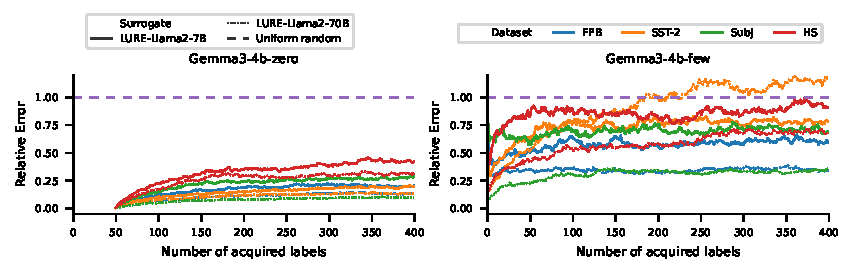
\includegraphics[width=0.9\linewidth, trim={15pt 5pt 0 0}]{ 
        figures/pdf/relative_errors_gemma_llama.pdf
    }
    \caption{
        Older Llama 2 models are useful surrogates for active testing of newer Gemma 3 target models.
    }
    \label{fig:relative_errors_gemma_llama}
\end{figure*}
\begin{figure*}[t]
    \centering
    % trim={<left> <lower> <right> <upper>}
    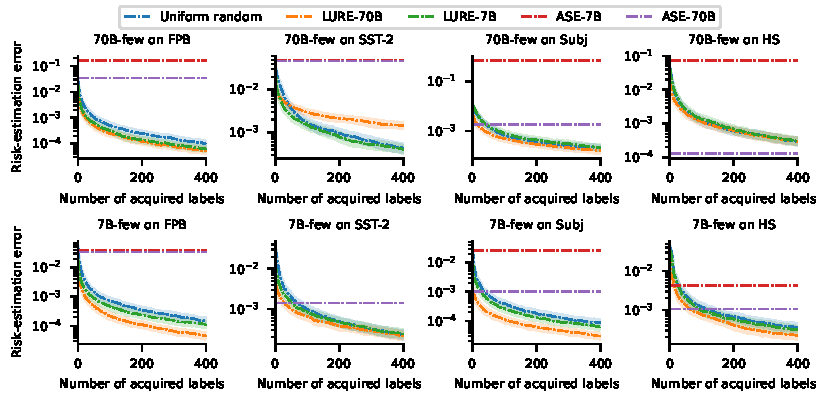
\includegraphics[width=0.95\linewidth,trim={0 5pt 0 0}]{
        figures/pdf/7b_70b_fewshot_lure_ase.pdf
    }
    \caption{
        Our sampling-based active testing (LURE) approach works more reliably than interpolation-based active testing (ASE) when using cheaply constructed surrogate models.
        In ASE the surrogate model not only guides data acquisition but also much more directly affects the risk estimate: the labels used to compute the expected loss of the target model are simulated from the surrogate model.
    }
    \label{fig:7b_70b_fewshot_lure_ase}
    \vspace{-8pt}
\end{figure*}


\subsection{Small surrogate models can be used to evaluate larger target models}

A key additional result to highlight in \Cref{fig:7b_70b_llama_unif_lure} is that LURE-7B works well not just for evaluating a target model of the same size, but also for evaluating a target model ten times larger.
In fact, we show that we can reduce surrogate-model costs even further by using Gemma3-4B (\Cref{fig:7b_70b_gemma_unif_lure}) and Phi-2 (\Cref{fig:7b_70b_phi_unif_lure}) to evaluate Llama 2 models, reducing computational costs by using even smaller surrogates.
Meanwhile, older Llama 2 models effectively evaluate newer Gemma 3 models (\Cref{fig:relative_errors_gemma_llama}), which perform strongly on these datasets (\Cref{tab:loss_models,tab:accuracy_models}).
As discussed in \Cref{sec:surrogate_prediction}, this ability to use a small surrogate model---combined with the fact that fixing the surrogate model allows us to only compute one forward pass on the pool set---is a useful way of reducing costs.


\subsection{Using stripped-back surrogate models favours sampling-based active testing}

Next we evaluate our claim in \Cref{sec:surrogate_training} that sampling-based active testing is preferable over interpolation-based active testing given that the surrogate model is fixed.
We do this by comparing our approach with ASE in evaluating the 7B-few and 70B-few models. 
Our results show ASE produces strong results on the HS dataset with the 70B-few model, but otherwise significantly underperforms (\Cref{fig:7b_70b_fewshot_lure_ase}).
This is consistent with our explanation that ASE is more sensitive to the quality of the surrogate model, and that computational constraints on the surrogate model make it less practically useful.
Note that the ASE risk estimator is constant if the surrogate model is fixed, as it is here.


\subsection{Good data acquisition is possible without making predictions with the target model}\label{sec:entropy_acquisition}

Now we explore our suggestion in \Cref{sec:target_prediction} that the surrogate model can be used to approximate the target model, such that we do not require target-model predictions during data acquisition.
For the logarithmic loss we are using, this equates to using the predictive entropy of the surrogate model as the acquisition function.
We assess this approach as applied to evaluating the 70B-few model with LURE-7B, and find it is surprisingly effective (\Cref{fig:70b_fewshot_entropy_relative_error}).
This is promising: it suggests all the cost-reduction measures proposed in \Cref{sec:scaling_method} are compatible with strong active-testing performance.


\begin{figure}[t]
    \centering
    \begin{minipage}[t]{0.48\textwidth}
        \centering
        % trim={<left> <lower> <right> <upper>}
        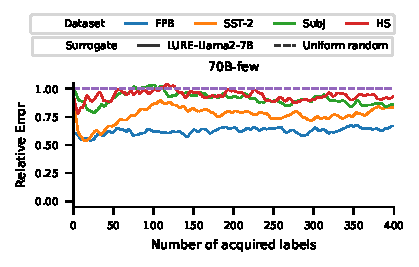
\includegraphics[width=\linewidth,trim={0 5pt 0 0}]{
            figures/pdf/70b_fewshot_entropy_relative_error.pdf
        }
        \caption{
            Using the surrogate model to approximate the target model during data acquisition (here this means acquiring data based on the predictive entropy of the surrogate model) reduces the need for target-model predictions while still performing well.
        }
        \label{fig:70b_fewshot_entropy_relative_error}
    \end{minipage}
    \hfill
    \begin{minipage}[t]{0.48\textwidth}
        \centering
        % trim={<left> <lower> <right> <upper>}
        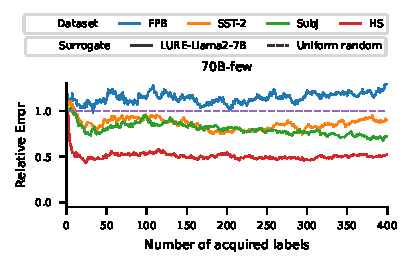
\includegraphics[width=\linewidth,trim={0 5pt 0 0}]{
            figures/pdf/70b_fewshot_nll_relative_error.pdf
        }
        \caption{
            Active testing with a label-aware acquisition function (here the negative log likelihood of the surrogate model) enables dataset curation (selecting a subset of already-labelled test data) tailored to a target model of interest, helping reduce computational costs.
        }
        \label{fig:70b_fewshot_nll_relative_error}
    \end{minipage}
    \vspace{-5pt}
\end{figure}


\subsection{Active testing for dataset curation works, suggesting scope to reduce computational costs}\label{sec:dataset_curation}

Here we consider the alternative problem setting discussed in \Cref{sec:dataset_curation_method}, where the inputs in the pool set are already labelled but it is too expensive to compute target-model predictions on all of them, with a possible solution being to curate a subset using a cheap surrogate model.
More concretely we run active testing using the negative log likelihood as our label-aware acquisition function (\Cref{eq:label_aware_acq_fn}).

We find our approach improves over uniform-random subsampling on three datasets out of four (SST-2, Subj and HS) and performs slightly worse on FPB (\Cref{fig:70b_fewshot_nll_relative_error}).
These overall-positive results---along with those for the predictive-entropy function we considered in \Cref{sec:entropy_acquisition}---suggest that active testing could be a useful tool for dataset curation, reducing computational costs when using existing evaluation datasets.
The practical benefits of this could be significant: \citet{liang2023holistic} required almost 20,000 hours of (Nvidia A100) GPU hours to evaluate 30 models on their HELM benchmark.


\subsection{The benefit of active testing tends to hold in more challenging scenarios}\label{sec:mmlu}

Next we use the MMLU dataset to assess the robustness of active testing to an increase in task difficulty, which corresponds to worse surrogate-model performance (\Cref{tab:loss_models,tab:accuracy_models}) and thus poses a challenge for effective data acquisition.
Our results show active testing continuing to outperform uniform-random testing for most combinations of surrogate and target models, with the only failure occurring when using 70B-few for both the surrogate and target models (\Cref{fig:7b_70b_mmlu_unif_lure}).


\begin{figure*}[t]
    \centering
    % trim={<left> <lower> <right> <upper>}
    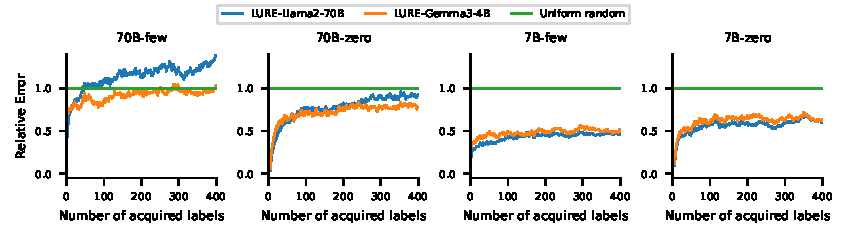
\includegraphics[width=\linewidth,trim={0 5pt 0 0}]{
        figures/pdf/relative_errors_full_mmlu.pdf
    }
    \caption{
        Active testing outperforms uniform-random testing in most cases on the harder MMLU dataset.
    }
    \label{fig:7b_70b_mmlu_unif_lure}
\end{figure*}
\begin{figure}[t]
    \centering
    % trim={<left> <lower> <right> <upper>}
    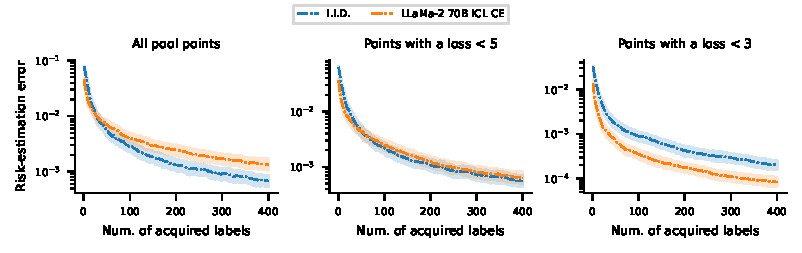
\includegraphics[width=0.95\linewidth,trim={0 5pt 0 0}]{
        figures/pdf/70b_fewshot_filtered_pool_sst.pdf
    }
    \caption{
        The failure of LURE-70B in efficiently evaluating the 70B-few model on the SST-2 dataset (left) is resolved by filtering incorrectly labelled datapoints from the pool set (middle, right).
        Underlying this effect is the presence of incorrect labels in the original dataset: we find that inputs with high loss are often mislabelled.
    }
    \label{fig:70b_fewshot_filtered_pool}
    \vspace{-8pt}
\end{figure}


\subsection{Incorrect labels can cause problems for active testing}\label{sec:failure}

Now we investigate the failure of LURE-70B to effectively evaluate the 70B-few model on the SST-2 dataset (\Cref{sec:basic_surrogates_work}).
We construct two modified versions of the SST-2 pool set: one filtered to remove inputs for which 70B-few's negative log likelihood (NLL) is greater than 5, and one filtered with a NLL threshold of 3.
Then we re-run active testing with these modified pool sets.

We show that the failure case is reduced by the weaker filtering and completely resolved by the stronger filtering (\Cref{fig:70b_fewshot_filtered_pool}).
To understand why, we inspect the filtered-out data and find it is often mislabelled.
We find 75\% of the 45 examples with NLL greater than 5 are mislabelled, and 67\% of the 136 examples with NLL greater than 3.
This is a useful demonstration of how active testing can fail when the source of labels is unreliable.
Interestingly it can also be seen as a case for using less powerful surrogate models to guide data acquisition: LURE-7B worked well in the exact case where LURE-70B failed.
It is also worth noting that in a dataset-curation setting (\Cref{sec:dataset_curation}) we have access to all the test labels and therefore have the option to directly filter out high-NLL examples.


\begin{figure*}[t]
    \centering
    % trim={<left> <lower> <right> <upper>}
    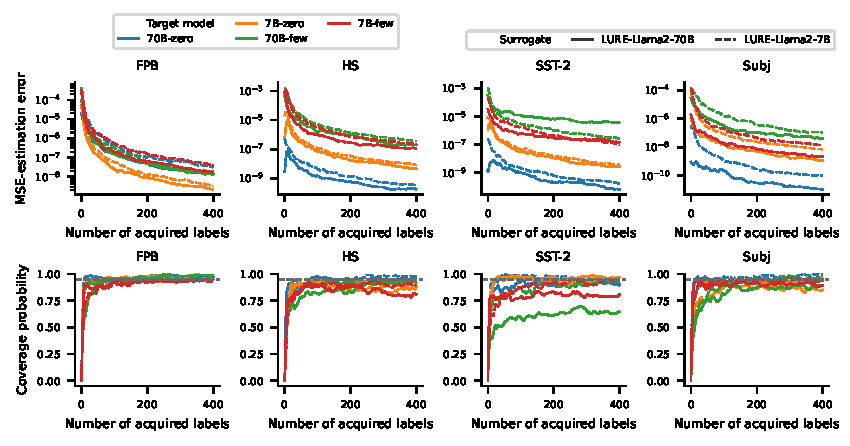
\includegraphics[width=\linewidth,trim={0 5pt 0 0}]{
        figures/pdf/error_estimation.pdf
    }
    \caption{
        Our bootstrap estimator of the active-testing risk-estimation error provides a useful performance indicator.
        Coverage probability measures how often a confidence interval contains the true risk-estimation error.
    }
    \label{fig:error_estimation}
\end{figure*}


\subsection{Bootstrap estimation of risk-estimation error provides an accurate performance indicator}\label{sec:boot}

Having assessed our proposed active-testing method, we turn to our method for estimating the mean squared error of the LURE risk estimator (\Cref{sec:error_estimation_method}).
We run active testing $T=100$ times, generating 100 sequences of acquired indices, $(i_{1:M})_{j=1}^{100}$.
Then for $K \in \{1, 2, \ldots, M\}$ we perform four steps:

\begin{enumerate}
    \item Compute a ground-truth mean-squared error, $\mathrm{MSE}_K$, using \Cref{eq:mse_decomposition} with $q(i_{1:K})$ defined as a uniform distribution over the $K$ index sequences acquired so far.
    \item Compute a bootstrap estimate of the MSE, $\widehat{\mathrm{MSE}}_K$, using \Cref{eq:variance_estimator} with $B=1000$ estimates.
    \item Compute the MSE-estimation error, $(\mathrm{MSE}_K - \widehat{\mathrm{MSE}}_K)^2$.
    \item Compute an approximate confidence interval, $\widehat{\mathrm{MSE}}_K \pm 2 \hat{\sigma}$, using estimated standard deviation $\hat{\sigma}$.
\end{enumerate}

Our results show MSE-estimation error converging to low values for most runs, after an initial period ($K<100$) of relatively high error (\Cref{fig:error_estimation}).
In addition to this, our confidence intervals provide high levels of coverage: for a strong majority of runs we see coverage probabilities of around 94\% for $K\geq 100$, suggesting a practitioner can expect their computed confidence interval to contain the true mean squared error approximately 94\% of the time.
While there are cases where MSE estimation fails, the overall performance is promising, suggesting our proposed method could be a useful practical performance indicator, helping justify real-world deployment of active testing.